\documentclass[a2paper, 12pt]{article}
\usepackage[font={huge, bf}]{caption}
\usepackage{fontspec}
\setmainfont{Arial}
\usepackage{subcaption}
\usepackage{graphicx}
\usepackage{tikz}
\usepackage{tikzsymbols}
\usetikzlibrary{calc,patterns,shapes.geometric}
\usepackage{float}
\usepackage{pdflscape}
\usepackage{geometry}
\geometry{landscape, margin=2cm}
\captionsetup[subfigure]{justification=justified,singlelinecheck=false}
\pagestyle{empty}

\def\centerarc[#1](#2)(#3:#4:#5){\draw[#1] ($(#2)+({#5*cos(#3)},{#5*sin(#3)})$) arc (#3:#4:#5);}

\begin{document}
	\vspace*{\fill}
	\begin{figure}[!htbp]
		\centering
		\begin{subfigure}[b]{0.48\textwidth}
			\caption{Figure 1}
			\centering
			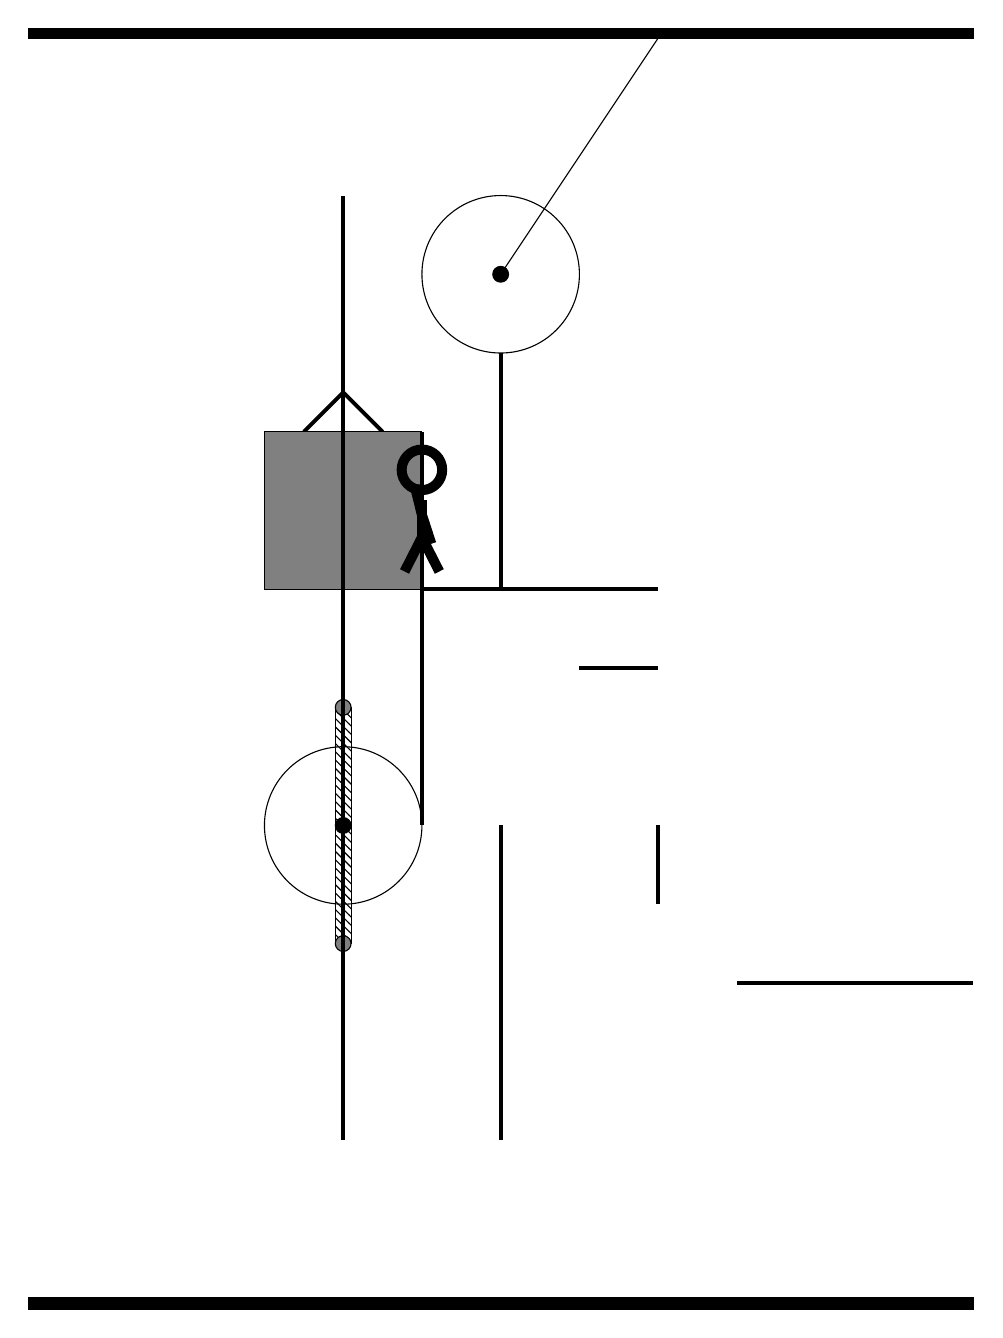
\begin{tikzpicture}
				\draw[fill=black] (-4, 14) rectangle (8, 14.125);
				
				\draw (2,11) circle (1);
				\draw[fill=black] (2,11) circle (0.1);
				\draw (4,14.0) -- (2,11);
				
				\draw (0,4) circle (1);
				\draw[fill=black] (0,4) circle (0.1);
				\draw[pattern=north west lines, pattern color=black] (-0.1,5.5) rectangle (0.1,2.5);
				\draw[fill=black!50] (0,5.5) circle (0.1);
				\draw[fill=black!50] (0,2.5) circle (0.1);
				
				\draw[line width=0.5mm](0,9.5) -- (0,12.0);
				\draw[line width=0.5mm](-0.5,9) --  (0,9.5) -- (0.5,9);
				\draw[fill=black!50] (-1, 9) rectangle (1, 7);
				
				\draw[line width = 0.5mm] (0,5) -- (0,10);
				\centerarc[line width = 0.5mm](1,10)(0:180:1);
				\draw[line width = 0.5mm] (2,10) -- (2,7);
				\centerarc[line width = 0.5mm](3,7)(270:180:1);
				\draw[line width = 0.5mm] (3,6) -- (4,6);
				\draw[line width = 0.5mm] (1,7) -- (4,7);
				\centerarc[line width = 0.5mm](1,6)(90:180:1);
				\draw[line width = 0.5mm] (0,6) -- (0,0);
				\centerarc[line width = 0.5mm](1,0)(180:360:1);
				\draw[line width = 0.5mm] (2,0) -- (2,4);
				\centerarc[line width = 0.5mm](3,4)(0:180:1);
				\draw[line width = 0.5mm] (4,4) -- (4,3);
				\centerarc[line width = 0.5mm](5,3)(180:270:1);
				\draw[line width = 0.5mm] (5,2) -- (8,2);
				\draw[line width = 0.5mm] (1,4) -- (1,9);
				
				\node at (1, 8) {\scriptsize \Strichmaxerl[10][108][104]};
				
				\draw[fill=black] (-4, -2) rectangle (8, -2.15);
			\end{tikzpicture}
		\end{subfigure}
		\hfill
		\begin{subfigure}[b]{0.48\textwidth}
			\caption{Figure 2}
			\centering
			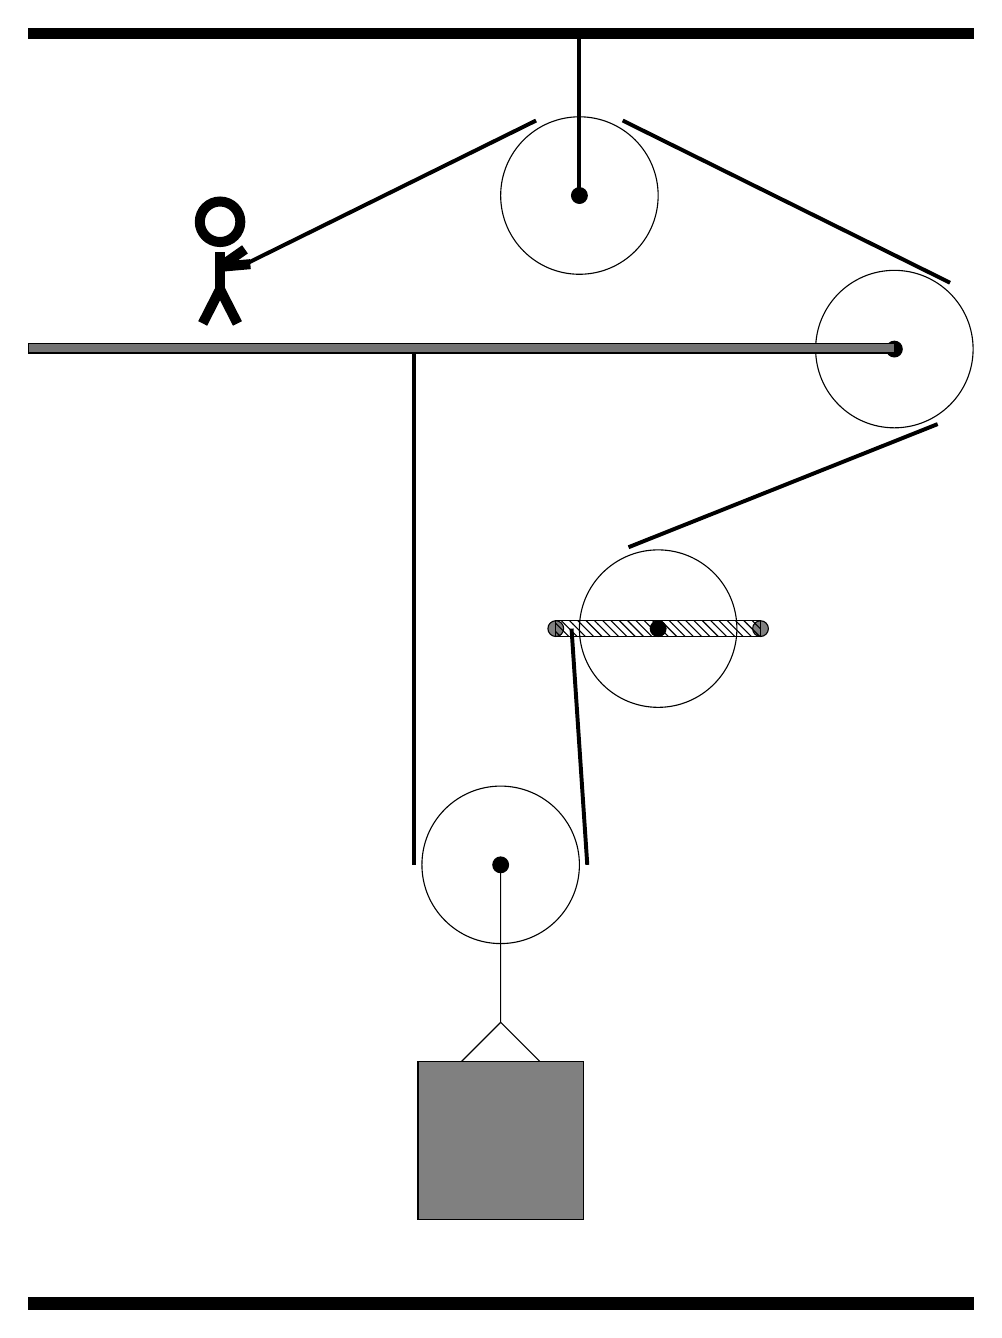
\begin{tikzpicture}
				\draw[fill=black] (-4, 14) rectangle (8, 14.125);
				
				\draw (2, 3.5) circle (1);
				\draw[fill=black] (2, 3.5) circle (0.1);
				
				\draw (7, 10.05) circle (1);
				\draw[fill=black] (7, 10.05) circle (0.1);
				
				\draw[fill=white](4, 6.5) circle (1);
				\draw[fill=black] (4, 6.5) circle (0.1);
				\draw[fill=black!50] (2.7, 6.5) circle (0.1);
				\draw[fill=black!50] (5.3, 6.5) circle (0.1);
				\draw[pattern=north west lines, pattern color=black] (2.7, 6.6) rectangle (5.3, 6.4);
				
				\draw (3, 12) circle (1);
				\draw[fill=black] (3, 12) circle (0.1);
				\draw[line width=0.5mm] (3, 12) -- (3, 14);
				
				\draw (2, 3.5) -- (2, 1.5) -- (1.5, 1.0) -- (2.5, 1.0) -- (2, 1.5);
				\draw[fill=black!50] (0.95, 1.0) rectangle (3.05, -1.0);
				
				\draw[line width=0.5mm] (0.9, 10) -- (0.9, 3.5);
				\centerarc[line width=0.5mm](2, 3.5)(180:360:1.1);
				\draw[line width=0.5mm](3.1, 3.5) -- (2.9, 6.5);
				\centerarc[line width=0.5mm](4, 6.5)(110:180:1.1);
				\draw[line width=0.5mm](3.6238, 7.5337) -- (7.55, 9.0974);
				\centerarc[line width=0.5mm](7, 10.05)(-60:50:1.1);
				\draw[line width=0.5mm](7.7071, 10.8926) -- (3.55, 12.9526);
				\centerarc[line width=0.5mm](3, 12)(60:120:1.1);
				\draw[line width=0.5mm](2.45, 12.9526) -- (-1.2, 11.15);
				
				\node at (-1.5, 11.15) {\footnotesize \scriptsize \Strichmaxerl[10][-175][35]};
				\draw[fill=black!55] (-4, 10) rectangle (7, 10.125);
				
				\draw[fill=black] (-4, -2) rectangle (8, -2.15);
			\end{tikzpicture}
		\end{subfigure}
	\end{figure}
		\vspace*{\fill}
\end{document}